\documentclass[acmsmall]{acmart}


\AtBeginDocument{%
  \providecommand\BibTeX{{%
    \normalfont B\kern-0.5em{\scshape i\kern-0.25em b}\kern-0.8em\TeX}}}


\begin{document}


\title{Automated Generation of Design Models from Source Code}


\author{yu Chen}
\author{shaoke Cui}
\author{xiaolei Gu}
\author{zeyu Han}
\author{wenfei Shi}
\author{weichen Zhang}


\begin{abstract}
Automated generation of design models from source code have shown promise as a cost-effective means for precise understanding of the system. In this paper, we conclude several challenges still exist in this field and find some research results corresponding to these challenges
\end{abstract}


\maketitle

\section{Introduction}


{\itshape Automated Generation of Design Models from Source Code} is a specific field of reverse engineering. It aims at generating design models from source code. The design models it generates can help developers understand the whole system, help evolve the system and check whether some behaviors of the system has errors. Since the scale and complexity of the system is increasing constantly, this technology becomes more and more significant.


According to the papers we have read, we have found some challenges exist in this field. The main aim of generating design models from source code is to help developers to understand how the system runs. So extracting business rules from source code is one of the basic challenge should meet. Also the design models should be smartly visualized to help developers have a specific understanding. Besides these basic needs, because of the large scale and complexity, it's time-consuming to finish this work. Complexity also causes possible information loss through transformation. Finally,considering multi-language program, the tools for generating design models should accept multi-language or transform multi-language to its own input language.

\section{Review Method}

\subsection{Research questions}
According to the main challenge mentioned above, we have raised five specific research questions.
\begin{itemize}
\item  How to extract the business logic from the source code
\item  How to visualize the design model for easier understanding
\item  How to solve the problem of time-consuming model construction and state explosion
\item  How to avoid the possible information loss when inferring relationships by attribute definition
\item  How to build tools that accept multi languages
\end{itemize}

\subsection{Search process}


    To find out the answer to these questions mentioned above, we used Google scholar, Baidu Scholar, 
    CNKI, wanfang, IEEEexplore and ACM database.
    Keywords such as reverse engineering, source code, graphic models,WCRE website ,ASE website,
    relationship pattern and UML were used.
    The criterion we took to include an particular research result is on fators such as
    its ranking on CCF's ranklist, its relationship to the question we raised which is indicated in the
    article's abstract.
    After the researching progress, the following articles were selected:\\
    \begin{tabular}{|c| p{5cm}|p{5cm}}
      question & title & author\\
      1&Reverse Engineering of Design Patterns from Java Source Code & Shi, N.  and  Olsson, R. A.\\
      1&Extracting business rules from COBOL: A model-based framework& Cosentino, V.  and  Cabot, J.\\
      2&Toward the Reverse Engineering of UML Sequence Diagrams for Distributed Java Software&Briand, Lionel C.  and  Labiche, Yvan  and  Leduc, Johanne\\
      2&On the use of metaballs to visually map source code structures and analysis results onto 3D space&Rilling, J.  and  Mudur, S. P.\\
      3&A deadlock detection tool for concurrent Java programs&DeMartini, Claudio and Iosif, Radu and Sisto, Riccardo\\
      3&Model checking java programs using java pathfinder&Havelund, Klaus and Pressburger, Thomas\\
      3&Bandera: Extracting finite-state models from Java source code&Corbett, James C and Dwyer, Matthew B and Hatcliff, John and Laubach, Shawn and Pasareanu, Corina S and Zheng, Hongjun and others\\
      4&Lightweight extraction of object models from bytecode&Jackson, D.  and  Waingold, A.\\
      5&A rule-based tool for reverse engineering from source code to graphical models&Huang, H.  and  Sugihara, K.  and  Miyamoto, I.\\
    \end{tabular}

\section{Review Result}

\subsection{extract the business logic from the source code}


Focusing on enhancing source code analysis tools by bringing program understanding to the design level. We found two different groups both have gone on the international success. They published their achievements on ASE and WCRE.

The first group come from Department of Computer Science, University of California\cite{2006Reverse}. They found that pattern definitions are either driven by code structure or system behavior. Based on this theory they reclassifying the GoF patterns to facilitate pattern recognition. Then they come up with two ways to detect patterns. One is detecting structure-driven patterns which can be identified by inter-class relationships. And the other is detecting behavior-driven patterns, such as template matching, which is often used in detecting malicious or buggy code. Based on the methodology above all, they implemented a fully automated pattern detection tool, called PINOT(Pattern INference recOvery Tool), built from Jikes. They claim that PINOT can recognizes all the GoF patterns in the structure and behavior-driven categories. 

While the other group solving the problem in a partly different way\cite{2014Extracting}. They put their eyes on COBOL, a procedural language that structures programs in 4 divisions: identification, environment, data and procedure divisions. The 4 divisions are used respectively to identify the program, to describe the input-ouput data sources, to declare the data structures and to define procedures to access and modify the program data structure. Based on the theory explained above and the principles of Model Driven Engineering, they describe a new BREX approach for COBOL applications. It has three steps including Variable Identification, Business Rule Identification and Business Rule Representation to extract business rules out of a COBOL application. The Variable Identification step reduces the number of variables to analyse by filtering out those that are not business relevant. It takes as input the COBOL model and returns the “business” variables. Business Rule Identification discovers the business rules related to the variables obtained in the Variable Identify step by static slicing techniques on the source code. Business Rule Representation is the last step of the framework. Its goal is to generate comprehensible textual and graphical representations of the discovered business rules and their orchestration.


The disadvantage of the first way is that its pattern recognition capability is not enough to recognize more complicated user-defined data structures. And the researchers didn’t explore the use of PINOT to detect design patterns in specific application domains.

And The second group haven’t complete the preliminary validation and cast the framework to practice. And the framework can be better with additional modules covering other technologies maximizing the reuse opportunities.


\subsection{visualize the design model for easier understanding}


Abstract representation of the source code is necessary in reverse engineering. But as programs become more complex and larger, developers need better ways to visualize the source code. Many visualization methods have been created to achieve this goal. Lionel's team create UML sequence diagrams for Java software by accounting for issues related to distribution \cite{2006Toward}. However, for large software systems UML diagrams will not provide adequate abstraction to visualize all the dependencies. So Juergen Rilling and S. P. Mudur use metaballs to visually map source code structures and analysis results onto 3D space \cite{2002On}.

Lionel's team first devises a metamodel of scenario diagrams that is an adaptation and simplification of the UML 2.0 metamodel for sequence diagrams . This helps them define the requirements in terms of information they need to retrieve from the traces, which will then drive their instrumentation. They formalize these requirements as a metamodel of traces. These metamodels are then used as follows: The execution of the instrumented SUS produces a trace, which is transformed into an instance of the trace metamodel. This trace metamodel instance is then transformed into an instance of the scenario diagram metamodel, using algorithms which are directly derived from consistency rules (or constraints) they define between the two metamodels. To simplify the definition of constraints on UML class diagrams, they use Object Constraint Language to describe the rules.

Metaballs, also known as metablobs, are a 3D object modeling technique which blends and transforms an assembly of particles with associated shapes into a more complex 3D shape. With the use of metaballs,  Juergen's team combines dynamic source analysis to selectively identify source code that is relevant at any point and combines it with 3D visualization techniques to reverse engineer and analyze source code, program executions, and program structures. Particles in the metaball metaphor can be mapped to software structures, with blobs representing an object or a function (distinguished by different shapes for particles) that are created dynamically during a program execution. The potential energy surrounding blobs has traditionally been used to indicate the influence amongst blobs. This can be very intuitively used to visualize the strength of the coupling among program artifacts. Besides, the dimensions or size of a blob can be used to indicate a desired measure of the software entity. The metaball metaphor provides a visually rich environment to depict entities in a software system along with visual techniques that enable mapping of software structure and dynamic behavior onto highly intuitive visual renderings. 


Some unstructured programming constructs can not be represented by UML 2.0 standard such as goto-like statements breaking out of multiple loop levels \cite{2006Toward}. So In the Lionel's paper, they assumed these constructs are not present in the source code. As programs become more complex and larger, Lionel's method isn't suitable for most of the software programs now. Extending their method by a extended UML standard is needed in translating source code into UML diagrams.

\subsection{solve the problem of time-consuming model construction and state explosion}


To attack the problem of model construction and state explosion of model checking technology, some make efforts to build a dedicated model checker for a specific programming language\cite{huch1999verification}. Others build tools such as JCAT \cite{demartini1999deadlock} 
and Java PathFinder \cite{havelund2000model},that translate a program directly into a relatively expressive verifier input language. 


Different from the above, Corbett's team uses a {\itshape component-based tool architecture for model extraction} which is called Bandera. The architecture of Bandera is like a compiler. It uses intermediate language called Jimple to stage the transformation from JAVA to model-checker input languages. It is built on {\itshape soot} compiler framework, using its own front-end called JJJC to maintain correspondence between a Java source program and its Jimple representation. 


Bandera uses three main methods to solve the problems, including component elimination, data abstraction, and component restriction. Component elimination means eliminate components irrelevant to the property being verified. One of the component of Bandera called Slicer is responsible for this. Date abstraction means abstract variables that contains unnecessary details to a smaller set that only contains necessary detail for verifying property. Abstraction-Based Specializer, also one of Bandera's components, provides automated support for reducing model size via data abstraction. It has an {\itshape abstraction library} indexed by concrete type correspond to an abstraction type. Users choose abstractions for relevant variables, then a type inference phase propagates this information and infers abstraction types for the remaining variables and for each expression in the program. Component restriction means when components can't be explictly eliminated or abstraction can't be defined, we can limit the number of components or set bounds among components to construct a {\itshape restrict model}. Although it can't capture all behaviors of the program, it's useful to find design errors in the program since many design errors are manifest in small versions of a system. Bandera uses a model-generator to setting bounds for various system components.


Besides the components mentioned above, Bandera also has Back End to take the sliced and abstracted program and produce verifier-specific representations for targeted verifiers.The back end components communicate through an intermediary between compiler-based representations and 
verifier-based representations called BIR. Through BIR, it's simple to  write translators for target verifiers because user only need to write a translator from BIR to the input language of the verifier. BIR contains some higher-level constructs to facilitate modeling Java so some constructs don't need to be removed. Instead, translators can implement these constructs in the most efficient in the verifier input language. This can help produce more compact models.


For the approaches mentioned above, they all have some limitations. For example, building a model checker for a specific language makes it difficult to keep the checking engine state-of-the-art and new methods for curbing the state explosion must be recoded in the tool’s dedicated engine\cite{corbett2000bandera}. Building translation tools may result in larger models due to mismatch between the semantics of the two languages. Bandera, although has advantage on scalability, flexibility and extensibility, it for now still can't handle all features of Java such as  interfaces or user-thrown exceptions.

\subsection{avoid the possible information loss when inferring relationships by attribute definition}


Previous methods has a crucial flaw.  Object models should not expose the representations of objects.
In case an one-to-many relationship for fileds represented as arrays, such as
an implementation of employees association with a vector:
\\
\\
\textbf{Vector employees;}
\\
\\This would result in an edge from Company to Vector , both
inappropriately exposing the representation of the
employees field and failing to show an association between
Company and Person.


To tackle the problem, Womble was an excellent tool\cite{2001Lightweight}.
With the following features, Womble does not suffer from this problem and
would still show an edge from Company to Person labeled
employees:
\begin{itemize}
    \item Associations are inferred by examining the methods
    of a class in addition to its declared fields. How a
    field is used provides more useful clues to its role
    than its declaration alone. Multiplicity and mutability of associations can both be determined.
    \item Container classes, such as Vector, are handled
    correctly most of the time: The container class does
    not appear as a node, but results in appropriate associations.
\end{itemize}


To extract UML from byte code, Womble makes use of most of the information in the
classfile. In particular, it uses the name of the class and the
names of classes it extends or implements, the declarations
of fields, static and virtual, the signatures of methods, and
the bytecode instructions within methods.


The basic structure of the object model is extracted as
follows: A node is introduced for each class, with a subset
edge for each extends or implements relationship. And,
roughly speaking, for each field declaration in a class A
of a field p of class B, an association labeled p from
A to B is added. Using its unique mechanism of inferring associations,
multiplicity and mutability.


 Womble uses a collection of simple heuristics to extract
object models from bytecode. The analysis is linear, mostly
monotonic (as classes are added), and reasonably accurate.
Despite its limitations,  it's an invaluable tool in our
everyday work.


Womble has several deficiencies. The major analysis flaw
is the inability to handle nested containers. It is quite
common, for example, for a class
C to have a field that is a
hashtable mapping strings to vectors of some other element
type E ; Womble fails to link C and E.
Womble also fails to
distinguish keys and values in a hashtable. Although
Womble's heuristics work well for many of the containers
that arise in practice, we have come to think that a more
systematic approach is needed.

\subsection{build tools that accept multi languages}


In recent years, some reverse engineering tools have been developed. However, they are oriented to software written in one specific programming language and extract only one or a few particular aspects of the software from source code. This limitation brings difficulties if the maintainers want to extract information from source code other than the information the tools provide. 

Hai Huang presents a rule-based tool MG (Model Generator)\cite{1992A} for reverse engineering from source code to graphical models defined in MERA (MetaEntity-Relation-Attribute) that is a uniform language for a variety of graphical models. MG enables maintainers to obtain the information they need and produce software specification in different models by specifying rules for generating it. It is also independent of programming languages in which source code is written. It is able to generate four graphical models: IOPM (Internal Operational Profile Model) representing control flow, EOPM (External Operational Profile Model) representing external behavior of a system, FSM (Functional Structure Model), UIM (User Interface Model).

A generation rule consists of two parts: Triggers and actions. A trigger indicates when the rule can be applied. Each rule may have one or more triggers. When any of the triggers in the rule has triggered, actions in the rule are executed sequentially. Each trigger has a set of conditions to be satisfied. The first one is a required condition called node type. It, indicates to which type of a node in the syntax tree the rule is applied.

Each rule has a set of actions which are executed sequentially. There are six types of actions: Graph, entity, relation, connect, process, and group. A graph action creates a graph. It takes four arguments - the name of the graph, formalism used in the graph, entry and exit entities of the graph. The scope of the graph action includes all the subsequent actions contained in the rule and all the subsequent actions executed before the next graph action is executed.

Use rule-based approach which can bring flexibility by explicitly representing the knowledge as rules of model generation. Any change of the knowledge only affects the rules that are much easier to modify than the tools themselves so that few modifications of the tool are needed. For a given graphical model formalism, generation rules describe how to translate each primitive element of a programming language into a piece of a diagram in the graphical model and how to assemble the produced pieces of diagrams and generate diagrams from them.

It is flexible to deal with different programming languages and extract various types of information from source code. The rule-based approach provides users with a means of customizing the tools so that the tools can deal with different programming languages and produce the models that the users want.


A limitation of MG is that it is difficult to generate a certain type of models such as CPM by using only the rule-based approach. The more expressive power the rules have, the more variety of models can be generated and at the same time the more complicated the rules are. Complicated rules lead to difficulties to create rules and to verify the rules. Due to these problems, the rules should not be complicated and hence the expressive power of rules should be limited to some extent.
\section{Conculsion}
In this research, we focused on the task {\itshape Automated generation of design models 
from source code have shown promise as a cost-effective means for precise understanding of the system.} 
In this paper, we conclude several challenges still exist in this field and find some research results 
corresponding to these challenges.


Toward {\itshape How to extract the business logic from the source code}, detecting structure-driven patterns which can be identified by
inter-class relationships and detecting behavior-driven patter is the 2 solutions we found.The disadvantage of the first way is that its pattern recognition capability is not enough to
recognize more complicated user-defined data structures. And The second group haven’t complete the preliminary validation and cast the framework to
practic.


Toward {\itshape visualize the design model for easier understanding}, we found 2 tools one is by Lionel's team and another is called Meataballs.


Toward {\itshape solve the problem of time-consuming model construction and state explosion}, Bandera and JCAT was detected.The architecture of Bandera is like a compile, and
 the first one  translate a program directly into a relatively expressive verifier input language.


 On {\itshape avoid the possible information loss when inferring relationships by attribute
 definition}, Womble was an incredible tool which tackle most of the circumstance where the problem might be met.
 Even though some drawback exists, it made a big contribution to this field and the tool is 
 well popular among related workers.


Finally, {\itshape build tools that accept multi language}, Hai Huang presents a rule-based tool MG (Model Generator) for reverse engineering from
source code to graphical models defined in MERA (MetaEntity-Relation-Attribute) that is a uniform language for a variety of graphical model.


There are many works dedicated to tackle the challenges in the field Automated generation of design models from source code have shown, through our investigation we deeply agree with that.
However, these tools and method metioned above have theri unique drawback to be solved.





\section{Reference}
\bibliographystyle{ACM-Reference-Format}
\bibliography{reference}

\section{Appendix}
Team leader: Wenfei Shi\\
Contributions: Yu Chen 100%, 
Shaoke Cui 100\%,
Xiaolei Gu 100\%,
Zeyu Han 100\%,
Wenfei Shi 100\%
Weichen Zhang 100\%.
\begin{figure}[h]
  \centerline{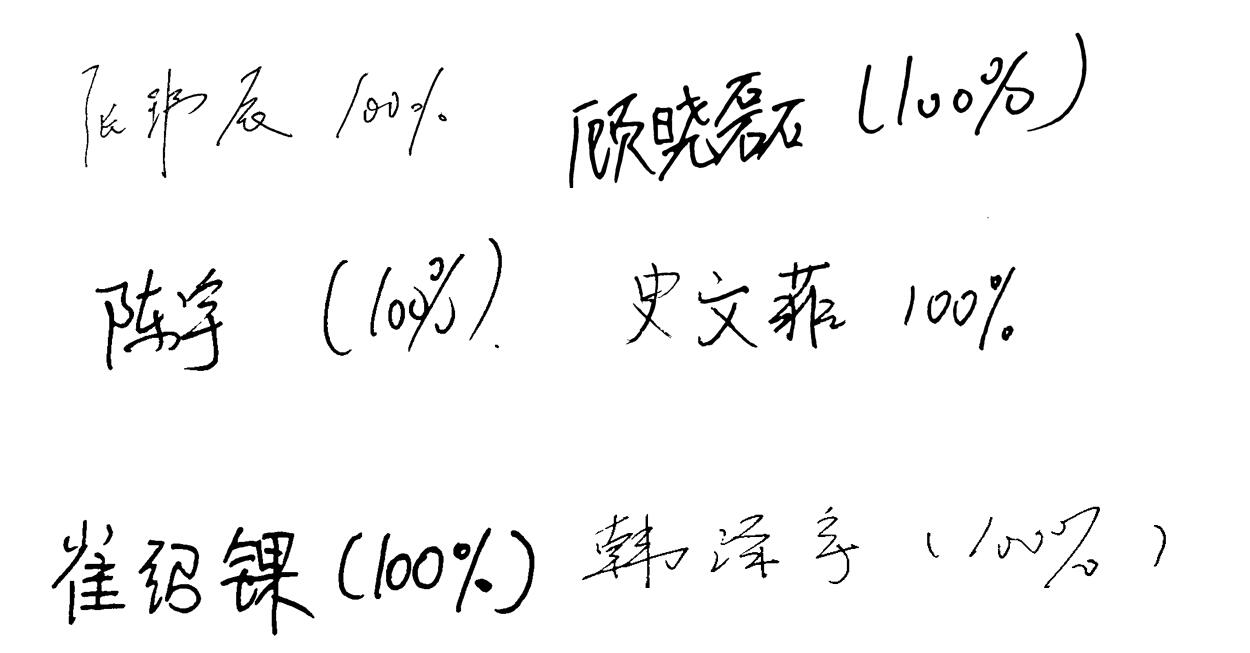
\includegraphics[scale=0.2]{signature.jpg}}
\end{figure}
\end{document}
\endinput